\chapter{Конструкторская часть}

В данном подразделе приводятся схемы разработанных алгоритмов, оценка их
трудоемкости, на основе которой производится оптимизация алгоритма Винограда с
последующим описаним алгоритма в виде схемы.

\section{Разработка алгоритмов стандартного \\
    умножения матриц и алгоритма Винограда}

\begin{figure}[h]
    \centering
    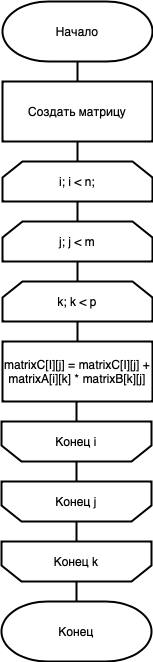
\includegraphics[width=0.21\linewidth]{img/standartAlg.jpg}
    \caption{Схема стандартного алгоритма умножения матриц}
    \label{fig:mpr}
\end{figure}

\begin{figure}[h]
    \centering
    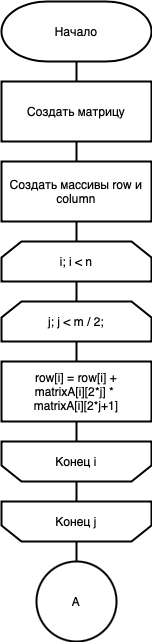
\includegraphics[width=0.3\linewidth]{img/WinogradPrA.jpg}
    \caption{Схема алгоритма Виноградова. Вычисление сумм роизведений 
    пар соседних элементов строк матрицы}
    \label{fig:mpr}
\end{figure}

\begin{figure}[h]
    \centering
    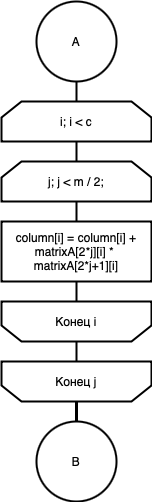
\includegraphics[width=0.3\linewidth]{img/WinogradPrB.jpg}
    \caption{Схема алгоритма Виноградова. Вычисление сумм роизведений 
    пар соседних элементов столбцов матрицы}
    \label{fig:mpr}
\end{figure}

\begin{figure}[h]
    \centering
    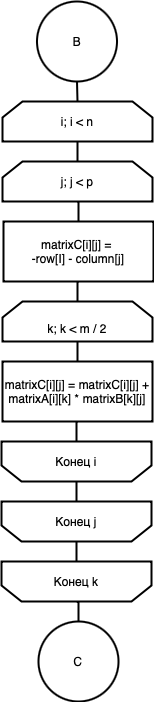
\includegraphics[width=0.3\linewidth]{img/WinogradPrC.jpg}
    \caption{Схема алгоритма Виноградова}
    \label{fig:mpr}
\end{figure}

\begin{figure}[h]
    \centering
    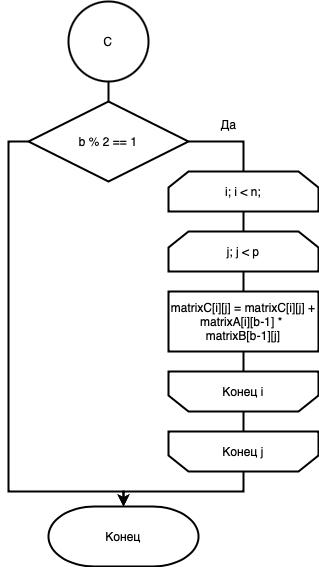
\includegraphics[width=0.6\linewidth]{img/WinogradPrD.jpg}
    \caption{Схема алгоритма Виноградова}
    \label{fig:mpr}
\end{figure}

\begin{figure}[h]
    \centering
    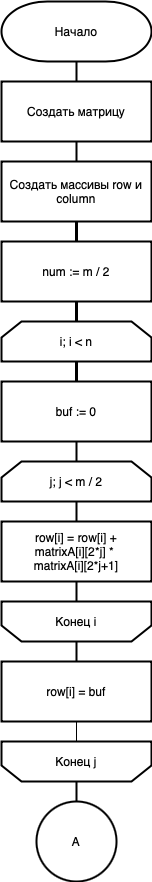
\includegraphics[width=0.25\linewidth]{img/WinogradOptA.jpg}
    \caption{Схема оптимизированного алгоритма Виноградова. Вычисление сумм роизведений 
    пар соседних элементов строк матрицы}
    \label{fig:mpr}
\end{figure}

\begin{figure}[h]
    \centering
    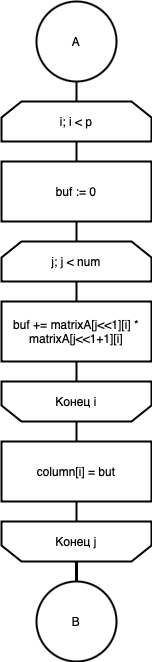
\includegraphics[width=0.3\linewidth]{img/WinogradOptB.jpg}
    \caption{Схема оптимизированного алгоритма Виноградова. Вычисление сумм роизведений 
    пар соседних элементов столбцов матрицы}
    \label{fig:mpr}
\end{figure}

\begin{figure}[h]
    \centering
    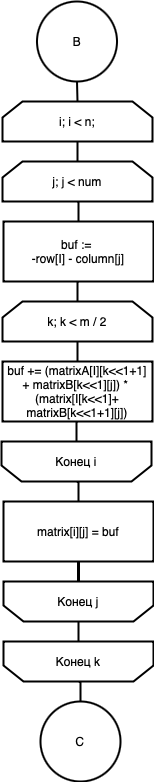
\includegraphics[width=0.3\linewidth]{img/WinogradOptC.jpg}
    \caption{Схема оптимизированного алгоритма Виноградова}
    \label{fig:mpr}
\end{figure}

\begin{figure}[h]
    \centering
    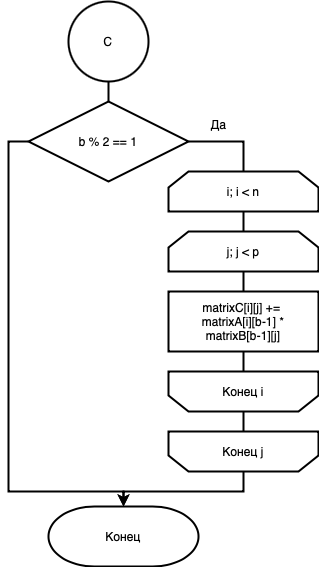
\includegraphics[width=0.6\linewidth]{img/WinogradOptD.jpg}
    \caption{Схема оптимизированного алгоритма Виноградова}
    \label{fig:mpr}
\end{figure}

\clearpage

\section{Модель вычислений для проведения оценки трудоемкости}

Введем модель вычислений, которая потребуется для определения 
трудоемкости каждого отдельного взятого алгоритма сортиров
\begin{enumerate}[label={\arabic*)}]
	\item Трудоемкость базовых операций имеет:
	\begin{itemize}[label=---]
		\item равную 1:
		\begin{equation}
			\label{for:operations_1}
			\begin{gathered}
				+, -, =, +=, -=, ==, !=, <, >, <=, >=, [], ++, {-}-,\\
				\&\&, >>, <<, ||, \&, |
			\end{gathered}
		\end{equation}
		\item равную 2:
		\begin{equation}
			\label{for:operations_2}
			*, /, \%, *=, /=, \%=
		\end{equation}
	\end{itemize}
	\item Трудоемкость условного оператора:
	\begin{equation}
		\label{for:if}
		f_{if} = f_{\text{условия}} + 
		\begin{cases}
			min(f_1, f_2), & \text{лучший случай}\\
			max(f_1, f_2), & \text{худший случай}
		\end{cases}
	\end{equation}
	\item Трудоемкость цикла:
	\begin{equation}
		\label{for:for}
		\begin{gathered}
			f_{for} = f_{\text{инициализация}} + f_{\text{сравнения}} + M_{\text{итераций}} \cdot (f_{\text{тело}} +\\
			+ f_{\text{инкремент}} + f_{\text{сравнения}})
		\end{gathered}
	\end{equation}
	\item Трудоемкость передачи параметра в функции и возврат из функции равны 0.
\end{enumerate}

\clearpage

\section{Оценка трудоемкости алгоритмов}

\subsection{Стандартный алгоритм}

Трудоемкость стандартного алгоритма умножения матриц считается следующим
образом:
\begin{itemize}[left=\parindent]
    \item трудоемкость цикла А вычисляется по формуле \ref{aeq};
        \begin{equation}\label{aeq}
            f_A = 1 + 1 + N(f_B + 1 + 1) = 2 + N(2 + f_B)
        \end{equation}
    \item трудоемкость цикла B вычисляется по формуле \ref{beq};
        \begin{equation}\label{beq}
            f_B = 1 + 1 + M(f_C + 1 + 1) = 2 + M(2 + f_C)
        \end{equation}
    \item трудоемкость цикла C вычисляется по формуле \ref{ceq};
        \begin{equation}\label{ceq}
            f_C = 1 + 1 + P(9 + 1 + 1) = 2 + 11P
        \end{equation}
\end{itemize}

Кроме циклов в стандартном алгоритме нет действий, поэтому трудоемкость
алгоритма равна трудоемкости внешнего цикла А и равна \ref{standarteq}:
\begin{equation}\label{standarteq}
    f_{standart} = 2 + N(2 + 2 + M(2 + 2 + 11P)) = 11NMP + 4MN + 4N + 2 
\end{equation}

\clearpage
\subsection{Алгоритм Виноградова}

Трудоемкость алгоритма умножения матриц Винограда считается следующим образом:
\begin{itemize}[left=\parindent]
    \item трудоемкость заполнения массива row вычисляется по формуле
        \begin{multline}\label{mulHeq}
            f_{row} = f_A = 2 + N(2 + f_B) = \\ = 2 + N(2 +
                       1 + 3 + \frac{P}{2}(3 + 1 + 15)) = \\ = 2 +
                       N(6 + \frac{19P}{2}) = 9.5PN + 6N + 2
        \end{multline}

    \item трудоемкость заполнения массива column вычисляется по формуле
        \begin{multline}\label{mulVeq}
            f_{column} = f_A = 2 + M(2 + f_B) = \\ = 2 +
            M(2 + 1 + 3 + \frac{P}{2}(1 + 3 + 15)) = \\ = 2 + M(6 +
            \frac{19P}{2}) = 9.5MP + 6M + 2
        \end{multline}
    
    \item трудоемкость основной части алгоритма равна
        \begin{multline}\label{winmainbesteq}
            f_{main} = f_A = 2 + N(2 + f_B) = \\ =  2 + N(2 + 2 + M(2
            + 7 + f_c)) = \\ = 2 + N(4 + M(9 + 4 + \frac{P}{2}(4 + 28))) =
            \\ = 16NMP + 13NM + 4N + 2
        \end{multline}

    \clearpage
    \item трудоемкость худщего случая при P - нечетная равна
        \begin{multline}\label{winmainworseeq}
            f_{neg} = f_A = 3 + 2 + N(2 + f_C) = \\ =  5 + N(2 + 2 + M(2 +
            14)) = \\ = 2 + N(4 + 16M) = \\ = 16MN + 4N + 5
        \end{multline}
\end{itemize}

Таким образом, трудоемкость алгоритма Винограда равна \ref{winogradbest} для
лучшего случая, \ref{winogradworse} -- для худшего.
\begin{multline}\label{winogradbest}
    f_{Winograd}^{\wedge} = 9.5NP + 6N + 2 +
                            9.5MP + 6M + 2 + 16NMP + 13NM + 4N + 2 = \\
                            = 16NMP + 13NM +9.5MP + 9.5NP + 10N + 6M + 6
\end{multline}
\begin{multline}\label{winogradworse}
    f_{Winograd}^{\vee} = 9.5NP + 6N + 2 + 9.5MP + 6M + 2 + 16NMP + \\
                            + 13NM + 4N + 2 + 16MN + 4N + 5 = \\
                        = 16NMP + 29NM +9.5NP + 9.5 MP + 14N + 6M + 11
\end{multline}


\section{Оптимизация алгоритма Винограда}

Как видно по вычисленным трудоемкостям алгоритмов (формулы \ref{standarteq} и
\ref{winogradbest}), трудоемкость алгоритма умножения матриц не уменьшилась, а
даже увеличилась, связано это с тем, что с вынесением предварительных
вычислений возросло количество таких дорогостоящих операций, как умножение и
деление. Чтобы получить выигрыш от предварительных вычислений, необходимо
оптимизировать алгоритм, для чего используем следующие типы оптимизации:
\begin{itemize}[left=\parindent]
    \item большинство производимых умножений и делений происходит на 2, поэтому
          заменим их на побитовый сдвиг влево и вправо соответственно;
    \item заменим выражения вида \texttt{x = x + y} на выражения вида \texttt{x
        += y}, а выражения вида \texttt{x = x - y} на выражения вида \texttt{x
        -= y}, избавившись худшем случае от одной операции при каждой замене;
    \item добавим буфер, чтобы постоянно не обращаться к элементам матрицы по индексам;
    \item p / 2 при сравнении и b - 1 при индексации заменим переменными, полученными до циклов.
\end{itemize}

\subsection{Оптимизированный алгоритм Виноградова}

Трудоемкость оптимизированного алгоритма умножения матриц Винограда считается следующим образом:

\begin{itemize}[left=\parindent]
    \item трудоемкость заполнения массива row вычисляется по формуле
        \begin{multline}\label{mulHeq}
            f_{row} = f_A = 2 + N(2 + f_B) = \\ = 2 + N(2 +
                       1 + 2 + 2 + \frac{P}{2}(2 + 10)) = \\ = 2 +
                       N(7 + \frac{12P}{2}) = 6NP + 7N + 2
        \end{multline}

        \item трудоемкость заполнения массива row вычисляется по формуле
        \begin{multline}\label{mulHeq}
            f_{column} = f_A = 2 + N(2 + f_B) = \\ = 2 + N(2 +
                       1 + 2 + 2 + \frac{P}{2}(2 + 10)) = \\ = 2 +
                       N(7 + \frac{12P}{2}) = 6MP + 7M + 2
        \end{multline}
    
    \item трудоемкость основной части алгоритма равна
        \begin{multline}\label{winmainbesteq}
            f_{main} = f_A = 2 + N(2 + f_B) = \\ =  2 + N(2 + 2 + M(2
            + 10 + f_c)) = \\ = 2 + N(4 + M(12 + \frac{P}{2}(22))) =
            \\ = 11NMP + 12NM + 4N + 2
        \end{multline}

    \clearpage
    \item трудоемкость худщего случая при P - нечетная равна
        \begin{multline}\label{winmainworseeq}
            f_{neg} = f_A = 3 + 2 + 2 + N(2 + f_C) = \\ =  7 + N(2 + 2 + M(2 +
            9)) = \\ = 7 + N(4 + 11M) = \\ = 11MN + 4N + 7
        \end{multline}
\end{itemize}

Таким образом, трудоемкость алгоритма Винограда равна \ref{winogradbest} для
лучшего случая, \ref{winogradworse} -- для худшего.
\begin{multline}\label{winogradbest}
    f_{Winograd}^{\wedge} = 6NP + 7N + 2 + 6MP + 7M + 2 + \\
                            ÷+ 11NMP + 12NM + 4N + 2 = \\
                            = 11NMP + 12NM + 6MP + 6NP + 11N + 7M + 6
\end{multline}

\begin{multline}\label{winogradworse}
    f_{Winograd}^{\vee} = 6NP + 7N + 2 + 6MP + 7M + 2 + \\
                            + 11NMP + 12NM + 4N + 2 + 11MN + 4N + 7 = \\
                        = 11NMP + 23NM + 6MP + 6NP + 11N + 7M + 13
\end{multline}

\section{Описание используемых типов данных}

При реализации алгоритмов будут использованы следующие структуры данных:

\begin{itemize}
	\item количество строк --- целое число;
	\item количество столбцов --- целое число;
	\item матрица --- двумерный список целых чисел
\end{itemize}

\clearpage
\section{Вывод}

В данном разделе были разработаны алгоритмы умножения матриц: стандартный и Винограда, 
-- также была произведена оценка трудоемкостей алгоритмов и оптимизация алгоритма Винограда. 
Для дальшейшей проверки правильности работы программы были выделены классы эквавалентности тестов.

